%% This is the ctufit-thesis example file. It is used to produce theses
%% for submission to Czech Technical University, Faculty of Information Technology.
%%
%% This is version 1.3.0, built 17. 6. 2024.
%% 
%% Get the newest version from
%% https://gitlab.fit.cvut.cz/theses-templates/FITthesis-LaTeX
%%
%%
%% Copyright 2024, Tomas Novacek
%% Copyright 2021, Eliska Sestakova and Ondrej Guth
%%
%% This work may be distributed and/or modified under the
%% conditions of the LaTeX Project Public License, either version 1.3
%% of this license or (at your option) any later version.
%% The latest version of this license is in
%%  https://www.latex-project.org/lppl.txt
%% and version 1.3 or later is part of all distributions of LaTeX
%% version 2005/12/01 or later.
%%
%% This work has the LPPL maintenance status `maintained'.
%%
%% The current maintainer of this work is Tomas Novacek.
%% Alternatively, submit bug reports to the tracker at
%% https://gitlab.fit.cvut.cz/theses-templates/FITthesis-LaTeX/issues
%%
%%

% arara: pdflatex
% arara: biber
% arara: pdflatex
% arara: pdflatex

%%%%%%%%%%%%%%%%%%%%%%%%%%%%%%%%%%%%%%%%%
% CLASS OPTIONS
% language: czech/english/slovak
% thesis type: bachelor/master/dissertation
% colour: bw for black&white OR no option for default colour scheme
% electronic (oneside) or printed (twoside), twoside is default
%%%%%%%%%%%%%%%%%%%%%%%%%%%%%%%%%%%%%%%%%
\documentclass[czech,bachelor,unicode,oneside]{ctufit-thesis}

%%%%%%%%%%%%%%%%%%%%%%%%%%%%%%%%%%
% FILL IN THIS INFORMATION
%%%%%%%%%%%%%%%%%%%%%%%%%%%%%%%%%%
\ctufittitle{Název příkladné závěrečné práce} % replace with the title of your thesis
\ctufitauthorfull{Bc. Jiří Nebozíz} % replace with your full name (first name(s) and then family name(s) / surname(s)) including academic degrees
\ctufitauthorsurnames{Nebozíz} % replace with your surname(s) / family name(s)
\ctufitauthorgivennames{Jiří} % replace with your first name(s) / given name(s)
\ctufitsupervisor{doc.\,Ing.\,Damien Zlo,\,Ph.D.} % replace with name of your supervisor/advisor (include academic degrees)
\ctufitdepartment{Katedra teoretické informatiky} % replace with the department of your defence
\ctufityear{2021} % replace with the year of your defence
\ctufitdeclarationplace{Praze} % replace with the place where you sign the declaration
\ctufitdeclarationdate{\today} % replace with the date of signature of the declaration
\ctufitabstractCZE{Fill in the abstract of this thesis in Czech. Apakrychle lórencz ipsum dolor sit amet. Class aptent taciti sociosqu ad litora torquent per conubia nostra, per inceptos hymenaeos. Cras pede libero, dapibus nec, pretium sit amet, tempor quis. Sed vel lectus. Donec odio tempus molestie, porttitor ut, iaculis quis, sem. Suspendisse sagittis ultrices augue.}
\ctufitabstractENG{Fill in the abstract of this thesis in English. Apakrychle lórencz ipsum dolor sit amet. Class aptent taciti sociosqu ad litora torquent per conubia nostra, per inceptos hymenaeos. Cras pede libero, dapibus nec, pretium sit amet, tempor quis. Sed vel lectus. Donec odio tempus molestie, porttitor ut, iaculis quis, sem. Suspendisse sagittis ultrices augue.}
\ctufitkeywordsCZE{enter, comma, separated, list, of, keywords, in, CZECH}
\ctufitkeywordsENG{enter, comma, separated, list, of, keywords, in, ENGLISH}
%%%%%%%%%%%%%%%%%%%%%%%%%%%%%%%%%%
% END FILL IN
%%%%%%%%%%%%%%%%%%%%%%%%%%%%%%%%%%

%%%%%%%%%%%%%%%%%%%%%%%%%%%%%%%%%%
% CUSTOMIZATION of this template
% Skip this part or alter it if you know what you are doing.
%%%%%%%%%%%%%%%%%%%%%%%%%%%%%%%%%%

\RequirePackage{iftex}[2020/03/06]
\iftutex % XeLaTeX and LuaLaTeX
    \RequirePackage{ellipsis}[2020/05/22] %ellipsis workaround for XeLaTeX
\else
    \errmessage{Only compilation with XeLaTeX or LuaLaTeX is allowed}
\fi

% hyperlinks
\RequirePackage[pdfpagelayout=TwoPageRight,colorlinks=false,allcolors=decoration,pdfborder={0 0 0.1}]{hyperref}[2020-05-15]

% uncomment the following to hide all hyperlinks
%\hypersetup{hidelinks}

% uncomment the following to change the colour of all hyperlinks to CTU blue
%\hypersetup{allbordercolors=decoration}

\RequirePackage{pdfpages}[2020/01/28]

%%%%%%%%%%%%%%%%%%%%%%%%%%%%%%%%%%
% CUSTOMIZATION of this template END
%%%%%%%%%%%%%%%%%%%%%%%%%%%%%%%%%%


%%%%%%%%%%%%%%%%%%%%%%
% DEMO CONTENTS SETTINGS
% You may choose to modify this part.
%%%%%%%%%%%%%%%%%%%%%%
\usepackage{dirtree}
\usepackage{lipsum,tikz}
\usepackage[style=iso-numeric]{biblatex}
\addbibresource{text/bib-database.bib}
\usepackage{xurl}
\usepackage{listings} % typesetting of sources
%\usepackage{minted}
\usepackage{csquotes}

%%%%%%%%%%%%%%%%%%%%%%
% DEMO CONTENTS SETTINGS END
%%%%%%%%%%%%%%%%%%%%%%

\begin{document} 
\frontmatter\frontmatterinit % do not remove these two commands

\thispagestyle{empty}\cleardoublepage\maketitle % do not remove these three commands

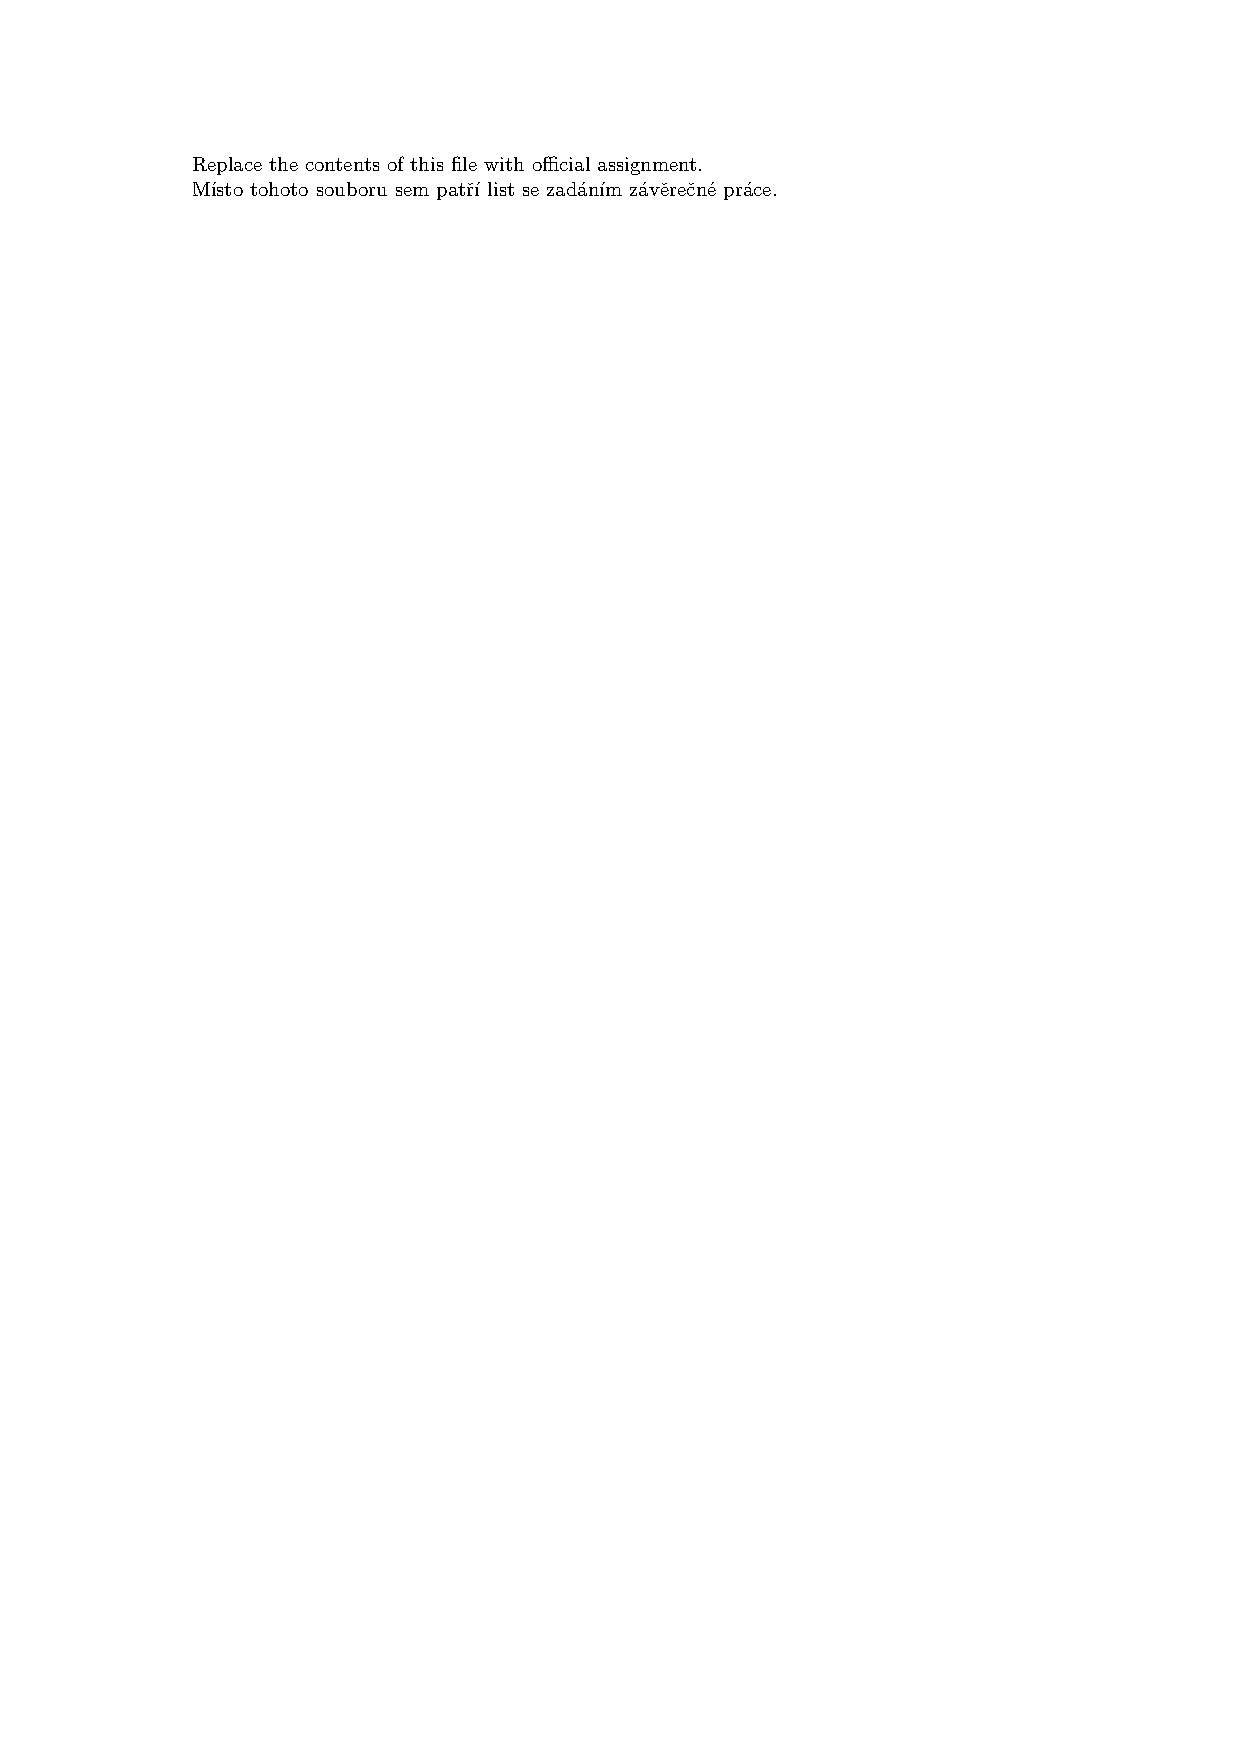
\includepdf[pages={1-}]{assignment-include.pdf} % replace this file with your thesis assignment generated from ProjectsFIT

\imprintpage % do not remove this command

\tableofcontents % do not remove this command
%%%%%%%%%%%%%%%%%%%%%%
% list of other contents: figures, tables, code listings, algorithms, etc.
% add/remove commands accordingly
%%%%%%%%%%%%%%%%%%%%%%
\listoffigures % list of figures
\begingroup
\let\clearpage\relax
\listoftables % list of tables
\thectufitlistingscommand
\endgroup
%%%%%%%%%%%%%%%%%%%%%%
% list of other contents END
%%%%%%%%%%%%%%%%%%%%%%

%%%%%%%%%%%%%%%%%%%
% ACKNOWLEDGMENT
% FILL IN / MODIFY
% This is a place to thank people for helping you. It is common to thank your supervisor.
%%%%%%%%%%%%%%%%%%%
\begin{acknowledgmentpage}
	Chtěl bych poděkovat především sit amet, consectetuer adipiscing elit. Curabitur sagittis hendrerit ante. Class aptent taciti sociosqu ad litora torquent per conubia nostra, per inceptos hymenaeos. Cras pede libero, dapibus nec, pretium sit amet, tempor quis. Sed vel lectus. Donec odio tempus molestie, porttitor ut, iaculis quis, sem. Suspendisse sagittis ultrices augue.
\end{acknowledgmentpage} 
%%%%%%%%%%%%%%%%%%%
% ACKNOWLEDGMENT END
%%%%%%%%%%%%%%%%%%%


%%%%%%%%%%%%%%%%%%%
% DECLARATION
% FILL IN / MODIFY
%%%%%%%%%%%%%%%%%%%
% INSTRUCTIONS
% ENG: choose one of approved texts of the declaration. DO NOT CREATE YOUR OWN. Find the approved texts at https://courses.fit.cvut.cz/SFE/download/index.html#_documents (document Declaration for FT in English)
% CZE/SLO: Vyberte jedno z fakultou schvalenych prohlaseni. NEVKLADEJTE VLASTNI TEXT. Schvalena prohlaseni najdete zde: https://courses.fit.cvut.cz/SZZ/dokumenty/index.html#_dokumenty (prohlášení do ZP)
\begin{declarationpage}
FILL IN ACCORDING TO THE INSTRUCTIONS. VYPLŇTE V SOULADU S POKYNY. Lorem ipsum dolor sit amet, consectetuer adipiscing elit. Curabitur sagittis hendrerit ante. Class aptent taciti sociosqu ad litora torquent per conubia nostra, per inceptos hymenaeos. Cras pede libero, dapibus nec, pretium sit amet, tempor quis. Sed vel lectus. Donec odio tempus molestie, porttitor ut, iaculis quis, sem. Suspendisse sagittis ultrices augue. Donec ipsum massa, ullamcorper in, auctor et, scelerisque sed, est. In sem justo, commodo ut, suscipit at, pharetra vitae, orci. Pellentesque pretium lectus id turpis.

Lorem ipsum dolor sit amet, consectetuer adipiscing elit. Curabitur sagittis hendrerit ante. Class aptent taciti sociosqu ad litora torquent per conubia nostra, per inceptos hymenaeos. Cras pede libero, dapibus nec, pretium sit amet, tempor quis. Sed vel lectus. Donec odio tempus molestie, porttitor ut, iaculis quis, sem. Suspendisse sagittis ultrices augue. Donec ipsum massa, ullamcorper in, auctor et, scelerisque sed, est. In sem justo, commodo ut, suscipit at, pharetra vitae, orci. Pellentesque pretium lectus id turpis.
\end{declarationpage}
%%%%%%%%%%%%%%%%%%%
% DECLARATION END
%%%%%%%%%%%%%%%%%%%

\printabstractpage % do not remove this command

%%%%%%%%%%%%%%%%%%%
% SUMMARY
% FILL IN / MODIFY
% OR REMOVE ENTIRELY (upon agreement with your supervisor)
% (appropriate to remove in most theses)
%%%%%%%%%%%%%%%%%%%
% \begin{summarypage}
% \section*{Summary section}
% 
% \lipsum[1][1-8]
% 
% \section*{Summary section}
% 
% \lipsum[2][1-6]
% 
% \section*{Summary section}
% 
% \lipsum[3]
% 
% \section*{Summary section}
% 
% \lipsum[2]
% 
% \section*{Summary section}
% 
% \lipsum[1][1-8] Lorem lorem lorem.
% \end{summarypage}
%%%%%%%%%%%%%%%%%%%
% SUMMARY END
%%%%%%%%%%%%%%%%%%%

%%%%%%%%%%%%%%%%%%%
% ABBREVIATIONS
% FILL IN / MODIFY
% OR REMOVE ENTIRELY
% List the abbreviations in lexicography order.
%%%%%%%%%%%%%%%%%%%
\chapter{\thectufitabbreviationlabel}
	
\begin{tabular}{rl}
DFA & Deterministic Finite Automaton\\
FA & Finite Automaton\\
LPS & Labelled Prüfer Sequence\\
NFA & Nondeterministic Finite Automaton\\
NPS & Numbered Prüfer Sequence\\
XML & Extensible Markup Language\\
XPath & XML Path Language\\
XSLT & eXtensible Stylesheet Language Transformations\\
W3C & World Wide Web Consortium
\end{tabular}
%%%%%%%%%%%%%%%%%%%
% ABBREVIATIONS END
%%%%%%%%%%%%%%%%%%%

\mainmatter\mainmatterinit % do not remove these two commands

%%%%%%%%%%%%%%%%%%%
% THE THESIS
% MODIFY ANYTHING BELOW THIS LINE
%%%%%%%%%%%%%%%%%%%

% Do not forget to include Introduction
%---------------------------------------------------------------
% \chapter{Introduction}
% uncomment the following line to create an unnumbered chapter
\chapter*{Introduction}\addcontentsline{toc}{chapter}{Introduction}\markboth{Introduction}{Introduction}
%---------------------------------------------------------------
\setcounter{page}{1}

% The following environment can be used as a mini-introduction for a chapter. Use that any way it pleases you (or comment it out). It can contain, for instance, a summary of the chapter. Or, there can be a quotation.
\begin{chapterabstract}
	\lipsum[1]
\end{chapterabstract}

\lipsum[2][1-4]{} [1]

\lipsum[4]

%---------------------------------------------------------------
\section{Ut enim ad minim veniam}
%---------------------------------------------------------------

\lipsum[6-7]

\begin{figure}
\centering
%\includegraphics[scale=0.4]{pic/index}
\resizebox{\textwidth}{!}{
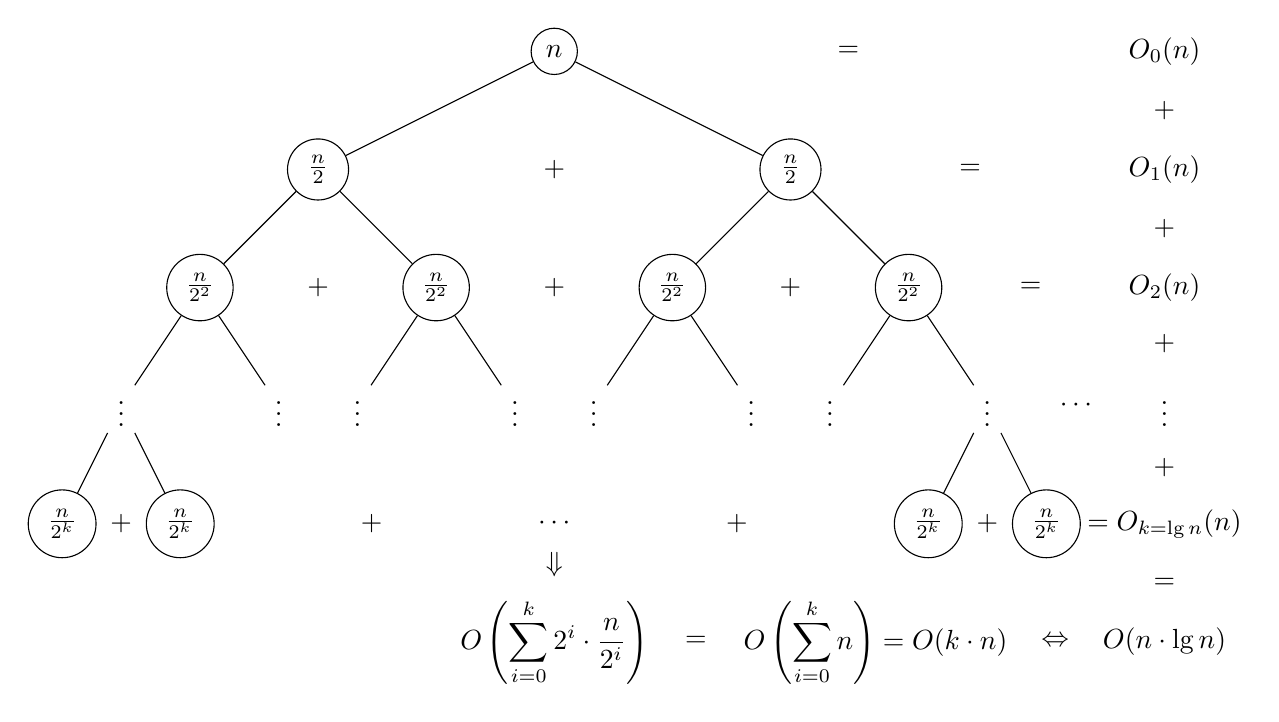
\begin{tikzpicture}[level/.style={sibling distance=60mm/#1}]
\node [circle,draw] (z){$n$}
  child {node [circle,draw] (a) {$\frac{n}{2}$}
    child {node [circle,draw] (b) {$\frac{n}{2^2}$}
      child {node {$\vdots$}
        child {node [circle,draw] (d) {$\frac{n}{2^k}$}}
        child {node [circle,draw] (e) {$\frac{n}{2^k}$}}
      } 
      child {node {$\vdots$}}
    }
    child {node [circle,draw] (g) {$\frac{n}{2^2}$}
      child {node {$\vdots$}}
      child {node {$\vdots$}}
    }
  }
  child {node [circle,draw] (j) {$\frac{n}{2}$}
    child {node [circle,draw] (k) {$\frac{n}{2^2}$}
      child {node {$\vdots$}}
      child {node {$\vdots$}}
    }
  child {node [circle,draw] (l) {$\frac{n}{2^2}$}
    child {node {$\vdots$}}
    child {node (c){$\vdots$}
      child {node [circle,draw] (o) {$\frac{n}{2^k}$}}
      child {node [circle,draw] (p) {$\frac{n}{2^k}$}
          child [grow=right] {node (q) {$ = O_{k = \lg n}(n)$} edge from parent[draw=none]
            child [grow=up] {node (r) {$\vdots$} edge from parent[draw=none]
              child [grow=up] {node (s) {$O_2(n)$} edge from parent[draw=none]
                child [grow=up] {node (t) {$O_1(n)$} edge from parent[draw=none]
                  child [grow=up] {node (u) {$O_0(n)$} edge from parent[draw=none]}
                }
              }
            }
            child [grow=down] {node (v) {$O(n \cdot \lg n)$}edge from parent[draw=none]}
        }
      }
    }
  }
};
\path (a) -- (j) node [midway] {+};
\path (b) -- (g) node [midway] {+};
\path (k) -- (l) node [midway] {+};
\path (k) -- (g) node [midway] {+};
\path (d) -- (e) node [midway] {+};
\path (o) -- (p) node [midway] {+};
\path (o) -- (e) node (x) [midway] {$\cdots$}
  child [grow=down] {
    node (y) {$O\left(\displaystyle\sum_{i = 0}^k 2^i \cdot \frac{n}{2^i}\right)$}
    edge from parent[draw=none]
  };
\path (q) -- (r) node [midway] {+};
\path (s) -- (r) node [midway] {+};
\path (s) -- (t) node [midway] {+};
\path (s) -- (l) node [midway] {=};
\path (t) -- (u) node [midway] {+};
\path (z) -- (u) node [midway] {=};
\path (j) -- (t) node [midway] {=};
\path (y) -- (x) node [midway] {$\Downarrow$};
\path (v) -- (y)
  node (w) [midway] {$O\left(\displaystyle\sum_{i = 0}^k n\right) = O(k \cdot n)$};
\path (q) -- (v) node [midway] {=};
\path (e) -- (x) node [midway] {+};
\path (o) -- (x) node [midway] {+};
\path (y) -- (w) node [midway] {$=$};
\path (v) -- (w) node [midway] {$\Leftrightarrow$};
\path (r) -- (c) node [midway] {$\cdots$};
\end{tikzpicture}}
\caption{~Lorem ipsum dolor sit amet}\label{img:index}
\end{figure}

%---------------------------------------------------------------
\section{Ut enim ad minim veniam}
%---------------------------------------------------------------

\lipsum[2-4]

%---------------------------------------------------------------
\subsection{Ut enim ad minim veniam}
%---------------------------------------------------------------

Curabitur ligula sapien, pulvinar a vestibulum quis, facilisis vel sapien. Duis condimentum augue id magna semper rutrum. Aliquam ornare wisi eu metus. Fusce aliquam vestibulum ipsum. Vivamus ac leo pretium faucibus\ref{img:index}.

\begin{itemize}
    \item Ut enim ad minim veniam, quis nostrud
    \item Ut enim ad minim 
    \item Ut enim ad minim veniam, quis 
    \begin{itemize}
        \item Ut enim ad
        \item Ut enim ad
        \begin{itemize}
            \item Ut enim 
            \item Ut enim 
            \begin{itemize}
            \item Ut enim 
            \item Ut enim 
        \end{itemize}
        \end{itemize}
    \end{itemize}
\end{itemize}

\section{Class aptent taciti}

\lipsum[2]

\subsection{Class aptent taciti}

\lipsum[6-7]

\begin{enumerate}
    \item Ut enim ad minim veniam, quis nostrud
    \item Ut enim ad minim 
    \item Ut enim ad minim veniam, quis 
    \begin{enumerate}
        \item Ut enim ad
        \item Ut enim ad
        \begin{enumerate}
            \item Ut enim 
            \item Ut enim 
            \begin{enumerate}
            \item Ut enim 
            \item Ut enim 
        \end{enumerate}
        \end{enumerate}
    \end{enumerate}
\end{enumerate}


%---------------------------------------------------------------
\section{Ut enim ad minim veniam, quis nostrud}
%---------------------------------------------------------------

Ut enim ad minim veniam, quis nostrud exercitation ullamco laboris nisi ut aliquip ex ea commodo consequat. Nulla non arcu lacinia neque faucibus fringilla. Vestibulum erat nulla, ullamcorper nec, rutrum non, nonummy ac, erat. Aliquam erat volutpat. Proin pede metus, vulputate nec, fermentum fringilla, vehicula vitae, justo.\footnote{Ut enim ad minim veniam, quis nostrud exercitation.} Etiam dictum tincidunt diam. In laoreet, magna id viverra tincidunt, sem odio bibendum justo, vel imperdiet sapien wisi sed libero. Nulla est. Maecenas fermentum, sem in pharetra pellentesque, velit turpis volutpat ante, in pharetra metus odio a lectus. Duis aute irure dolor in reprehenderit in voluptate velit esse cillum dolore eu fugiat nulla pariatur. 

\begin{lstlisting}[caption={~Zbytečný kód},label=list:8-6,captionpos=t,float,abovecaptionskip=-\medskipamount,belowcaptionskip=\medskipamount,language=C]
    #include<stdio.h>
    #include<iostream>
    // A comment
    int main(void)
    {
        printf("Hello World\n");
        return 0;
    }
\end{lstlisting}

%%%%%%%%%%%%%%%%%%%%%%%%%%%%%%%%%
% alternative using package minted for source highlighting
% package minted requires execution with `-shell-escape'
% e.g., `xelatex -shell-escape ctufit-thesis.tex'
% \begin{listing}
% \caption{Zbytečný kód}\label{list:8-6}
% \begin{minted}{C}
%     #include<stdio.h>
%     #include<iostream>
%     // A comment
%     int main(void)
%     {
%         printf("Hello World\n");
%         return 0;
%     }
% \end{minted}
% \end{listing}
% %%%%%%%%%%%%%%%%%%%%%%%%%%%%%%%%%
Nullam feugiat, turpis at pulvinar vulputate, erat libero tristique tellus, nec bibendum odio risus sit amet ante. Aenean id metus id velit ullamcorper pulvinar. Fusce wisi. Integer lacinia. Aliquam id dolor. Pellentesque pretium lectus id turpis. Suspendisse sagittis ultrices augue. In laoreet, magna id viverra tincidunt, sem odio bibendum justo, vel imperdiet sapien wisi sed libero. Sed ac dolor sit amet purus malesuada congue. \cite{Crochemore2002}

Class aptent taciti sociosqu ad litora torquent per conubia nostra, per inceptos hymenaeos. Fusce suscipit libero eget elit. Etiam dui sem, fermentum vitae, sagittis id, malesuada in, quam. Aliquam id dolor. Curabitur bibendum justo non orci. Duis viverra diam non justo. Curabitur ligula sapien, pulvinar a vestibulum quis, facilisis vel sapien. Duis condimentum augue id magna semper rutrum. Aliquam ornare wisi eu metus. Fusce aliquam vestibulum ipsum. Vivamus ac leo pretium faucibus. \cite{Motwani2014}

%---------------------------------------------------------------
\subsection{Ut enim ad minim veniam, quis nostrud}
%---------------------------------------------------------------

Ut enim ad minim veniam, quis nostrud exercitation ullamco laboris nisi ut aliquip ex ea commodo consequat. Nulla non arcu lacinia neque faucibus fringilla. Vestibulum erat nulla, ullamcorper nec, rutrum non, nonummy ac, erat. Aliquam erat volutpat. Proin pede metus, vulputate nec, fermentum fringilla, vehicula vitae, justo. Etiam dictum tincidunt diam. In laoreet, magna id viverra tincidunt, sem odio bibendum justo. \cite{Sestakova2018} 

\begin{table}\centering
\caption[Příklad tabulky]{~Zadávání matematiky}\label{tab:matematika}
\begin{tabular}{l|l|c|c}
	Typ		& Prostředí		& \LaTeX{}ovská zkratka	& \TeX{}ovská zkratka	\tabularnewline \hline 
 	Text		& \verb|math|		& \verb|\(...\)|	& \verb|$...$|	\tabularnewline \hline
 	Displayed	& \verb|displaymath|	& \verb|\[...\]|	& \verb|$$...$$|	\tabularnewline 
\end{tabular}
\end{table}


Nulla est. Maecenas fermentum, sem in pharetra pellentesque, velit turpis volutpat ante, in pharetra metus odio a lectus. Duis aute irure dolor in reprehenderit in voluptate velit esse cillum dolore eu fugiat nulla pariatur. Nullam feugiat, turpis at pulvinar vulputate, erat libero tristique tellus, nec bibendum odio risus sit amet ante. Aenean id metus id velit ullamcorper pulvinar. 

\subsubsection{Class aptent taciti}

\begin{definition}[Optional label]
Class aptent taciti sociosqu ad litora torquent per conubia nostra, per inceptos hymenaeos. Fusce suscipit libero eget elit. Etiam dui sem, fermentum vitae, sagittis id, malesuada in, quam. Aliquam id dolor. Curabitur bibendum justo non orci.
\end{definition}

\begin{example}
Class aptent taciti sociosqu ad litora torquent per conubia nostra, per inceptos hymenaeos. Fusce suscipit libero eget elit. Etiam dui sem, fermentum vitae, sagittis id, malesuada in, quam. Aliquam id dolor. Curabitur bibendum justo non orci.
\end{example}

\paragraph{Nadpis 5. úrovně}

\begin{theorem}
Class aptent taciti sociosqu ad litora torquent per conubia nostra, per inceptos hymenaeos. Fusce suscipit libero eget elit. Etiam dui sem, fermentum vitae, sagittis id, malesuada in, quam. Aliquam id dolor. Curabitur bibendum justo non orci.
\end{theorem}

\begin{proof}
Fusce suscipit libero eget elit. Etiam dui sem, fermentum vitae, sagittis id, malesuada in, quam. Aliquam id dolor. Curabitur bibendum justo non orci.
\end{proof}

\paragraph{Level 5 heading}

\begin{corollary}
Fusce suscipit libero eget elit. Etiam dui sem, fermentum vitae, sagittis id, malesuada in, quam. Aliquam id dolor. Curabitur bibendum justo non orci.
\end{corollary}

\begin{proposition}
Fusce suscipit libero eget elit. Etiam dui sem, fermentum vitae, sagittis id, malesuada in, quam. Aliquam id dolor. Curabitur bibendum justo non orci.
\end{proposition}

\begin{note}
Fusce suscipit libero eget elit. Etiam dui sem, fermentum vitae, sagittis id, malesuada in, quam. Aliquam id dolor. Curabitur bibendum justo non orci.
\end{note}

\begin{remark}
Fusce suscipit libero eget elit. Etiam dui sem, fermentum vitae, sagittis id, malesuada in, quam. Aliquam id dolor. Curabitur bibendum justo non orci.
\end{remark}

\begin{lemma}
Class aptent taciti sociosqu ad litora torquent per conubia nostra, per inceptos hymenaeos. Fusce suscipit libero eget elit. Etiam dui sem, fermentum vitae, sagittis id, malesuada in, quam. Aliquam id dolor. Curabitur bibendum justo non orci.
\end{lemma}

\lipsum[1-2]

% \subsection{Class aptent taciti sociosqu}
% 
% \lipsum[4-5]

%---------------------------------------------------------------
\chapter{Lorem ipsum}
%---------------------------------------------------------------

\begin{chapterabstract}
	Lorem ipsum dolor sit amet, consectetuer adipiscing elit. Curabitur sagittis hendrerit ante. Class aptent taciti sociosqu ad litora torquent per conubia nostra, per inceptos hymenaeos. Cras pede libero, dapibus nec, pretium sit amet, tempor quis. Sed vel lectus. Donec odio tempus molestie, porttitor ut, iaculis quis, sem. Cras pede libero, dapibus nec, pretium sit amet, tempor quis. Sed vel lectus. 
\end{chapterabstract}

Lorem ipsum dolor sit amet, consectetuer adipiscing elit. Curabitur sagittis hendrerit ante. Class aptent taciti sociosqu ad litora torquent per conubia nostra, per inceptos hymenaeos. Cras pede libero, dapibus nec, pretium sit amet, tempor quis. Sed vel lectus. Donec odio tempus molestie, porttitor ut, iaculis quis, sem. Suspendisse sagittis ultrices augue. Donec ipsum massa, ullamcorper in, auctor et, scelerisque sed, est. In sem justo, commodo ut, suscipit at, pharetra vitae, orci. Pellentesque pretium lectus id turpis. \cite{Kopka2004}

\section{Donec odio tempus molestie}

\lipsum[2] \cite{def:1, def:2}

\subsection{Class aptent taciti}

\lipsum[2-3]

\begin{description}
\item[Kapitola 1] Lorem ipsum dolor sit amet, consectetuer adipiscing elit. Curabitur sagittis hendrerit ante. Class aptent taciti sociosqu ad litora torquent per conubia nostra, per inceptos hymenaeos. Cras pede libero, dapibus nec, pretium sit amet, tempor quis.

\item[Kapitola 2] Lorem ipsum dolor sit amet, consectetuer adipiscing elit. Curabitur sagittis hendrerit ante. Class aptent taciti sociosqu ad litora torquent per conubia nostra, per inceptos hymenaeos. Cras pede libero, dapibus nec, pretium sit amet, tempor quis.

\item[Kapitola 3] Lorem ipsum dolor sit amet, consectetuer adipiscing elit. Curabitur sagittis hendrerit ante. Class aptent taciti sociosqu ad litora torquent per conubia nostra, per inceptos hymenaeos. Cras pede libero, dapibus nec, pretium sit amet, tempor quis.

\item[Kapitola 4] Lorem ipsum dolor sit amet, consectetuer adipiscing elit. Curabitur sagittis hendrerit ante. Class aptent taciti sociosqu ad litora torquent per conubia nostra, per inceptos hymenaeos. Cras pede libero, dapibus nec, pretium sit amet, tempor quis.
\end{description}

\lipsum[2]

\section{Lorem ipsum dolor sit amet}

\lipsum[3-5]
 % include `text.tex' from `text/' subdirectory

\appendix\appendixinit % do not remove these two commands

\chapter{Nějaká příloha}


Sem přijde to, co nepatří do hlavní části.
 % include `appendix.tex' from `text/' subdirectory

\backmatter % do not remove this command

\printbibliography % print out the BibLaTeX-generated bibliography list

\chapter{Obsah příloh}
% Contents of the attachment

	\dirtree{%
		.1 /.
		.2 readme.txt\DTcomment{stručný popis obsahu média}.
		.2 exe\DTcomment{adresář se spustitelnou formou implementace}.
		.2 src.
		.3 impl\DTcomment{zdrojové kódy implementace}.
		.3 thesis\DTcomment{zdrojová forma práce ve formátu \LaTeX{}}.
		.2 text\DTcomment{text práce}.
		.3 thesis.pdf\DTcomment{text práce ve formátu PDF}.
	}
 % include `medium.tex' from `text/' subdirectory

\end{document}
